\documentclass[12pt]{article}

\usepackage[T1]{fontenc}\usepackage{graphicx}\graphicspath{ {./images/} } \usepackage{float}\begin{document}

(Q)
Describe: ...
\clearpage
SCC361: Artificial Intelligence\\
Week 1: Introduction to Artificial Intelligence and Machine Learning\\
Dr Bryan M. Williams\\
School of Computing and Communications, Lancaster University\\
Office: InfoLab21 C40 Email: b.williams6@lancaster.ac.uk\\
1\\
\begin{figure}[H]

\includegraphics[width=0.5\linewidth]{page1-image-1.png}
\end{figure}
\clearpage
(Q)
Describe: ...
\clearpage
SCC361: Artificial Intelligence\\ 
\begin{figure}[H]

\includegraphics[width=0.5\linewidth]{page2-image-1.png}
\end{figure}
\clearpage
(Q)
Describe: questions
\clearpage
Playing this Video\\ 
\section{questions}
\begin{itemize}
  \item While watching, use the Questions? slides as stop points for 
coffee breaks, notes etc\\
\end{itemize}
3\\
\begin{figure}[H]

\includegraphics[width=0.5\linewidth]{page2-image-2.png}
\end{figure}
\clearpage
(Q)
Describe: is inaccessible in anyway to any individual or group, 
\clearpage
Accessibility\\ 
\section{is inaccessible in anyway to any individual or group, }
kindly let us know.\\
4\\
\begin{figure}[H]

\includegraphics[width=0.5\linewidth]{page2-image-3.png}
\end{figure}
\clearpage
(Q)
Describe: • Here is a the demo
\clearpage
Be sure to check in to all timetabled sessions using \\ 
\section{• Here is a the demo}
Please DO NOT leave a timetabled session without your\\
attendance being registered\\
Attendance Check-in\\
5\\
\begin{figure}[H]

\includegraphics[width=0.5\linewidth]{page2-image-4.png}
\end{figure}
\clearpage
(Q)
Describe: • Here is a the demo
\clearpage
Online Sessions on Teams\\ 
\begin{figure}[H]

\includegraphics[width=0.5\linewidth]{page2-image-5.png}
\end{figure}
\clearpage
(Q)
Describe: • Here is a the demo
\clearpage
Online Sessions on Teams\\ 
\begin{figure}[H]

\includegraphics[width=0.5\linewidth]{page2-image-6.png}
\end{figure}
\clearpage
(Q)
Describe: afterwards.
\clearpage
Online Sessions on Teams\\ 
\section{afterwards.}
Post additional questions on the SCC361 Moodle Forum\\
8\\
\begin{figure}[H]

\includegraphics[width=0.5\linewidth]{page2-image-7.png}
\end{figure}
\clearpage
(Q)
Describe: afterwards.
\clearpage
Online Sessions on Teams\\ 
\begin{figure}[H]

\includegraphics[width=0.5\linewidth]{page2-image-8.png}
\end{figure}
\clearpage
(Q)
Describe: Note:
\clearpage
The lectures can be watched on the Moodle space.\\ 
\section{Note:}
All learning materials: slides, videos and caption\\
files are @Lancaster University copyright and are \\
not to be shared or distributed.\\
Using Materials Offline\\
10\\
\begin{figure}[H]

\includegraphics[width=0.5\linewidth]{page2-image-9.png}
\end{figure}
\clearpage
(Q)
Describe: Plagiarism
\clearpage
Passing off someone else’s work as your own, including:\\ 
\section{Plagiarism}
11\\
\begin{figure}[H]

\includegraphics[width=0.5\linewidth]{page2-image-10.png}
\end{figure}
\clearpage
(Q)
Describe: Online Learning Expectations
\clearpage
• Online tools will be used to facilitate some aspects of learning e.g. Moodle, Teams, etc.\\ 
\section{Online Learning Expectations}
12\\
\begin{figure}[H]

\includegraphics[width=0.5\linewidth]{page3-image-1.png}
\end{figure}
\clearpage
(Q)
Describe: • However, we are asking that you use them sensibly and with respect
\clearpage
• Don’t forget, these are your fellow students and staff, not some anonymous person on \\ 
\section{• However, we are asking that you use them sensibly and with respect}
Online Learning Expectations\\
13\\
\begin{figure}[H]

\includegraphics[width=0.5\linewidth]{page3-image-2.png}
\end{figure}
\clearpage
(Q)
Describe: • Have a study plan, get a study partner
\clearpage
Attendance:\\ 
\section{• Have a study plan, get a study partner}
Integrity:\\
\end{itemize}
  \item Honesty, no plagiarism/ result manipulation
What do we expect from you?\\
\end{itemize}
14\\
\begin{figure}[H]

\includegraphics[width=0.5\linewidth]{page3-image-3.png}
\end{figure}
\clearpage
(Q)
Describe: • We encourage you to maximise the use of lab sessions for all coursework related 
\clearpage
• Lecture slides and videos will be available on Moodle\\ 
\section{• We encourage you to maximise the use of lab sessions for all coursework related }
questions\\
How can we help?\\
15\\
\begin{figure}[H]

\includegraphics[width=0.5\linewidth]{page4-image-1.png}
\end{figure}
\clearpage
(Q)
Describe: 16
\clearpage
• Use the labs to ask TAs/Tutors for help\\ 
\section{16}
\begin{figure}[H]

\includegraphics[width=0.5\linewidth]{page4-image-2.png}
\end{figure}
\clearpage
(Q)
Describe: 16
\clearpage
Questions?\\ 
\begin{figure}[H]

\includegraphics[width=0.5\linewidth]{page4-image-3.png}
\end{figure}
\clearpage
(Q)
Describe: 16
\clearpage
SCC361: Artificial Intelligence\\ 
\begin{figure}[H]

\includegraphics[width=0.5\linewidth]{page5-image-1.png}
\end{figure}
\clearpage
(Q)
Describe: 19
\clearpage
In this video\\ 
\section{19}
\begin{figure}[H]

\includegraphics[width=0.5\linewidth]{page5-image-2.png}
\end{figure}
\clearpage
(Q)
Describe: • learn how to evaluate the performance of AI systems
\clearpage
Expected Learning Outcomes\\ 
\section{• learn how to evaluate the performance of AI systems}
20\\
\begin{figure}[H]

\includegraphics[width=0.5\linewidth]{page5-image-3.png}
\end{figure}
\clearpage
(Q)
Describe: Module Convenor
\clearpage
Teaching Staff\\ 
\section{Module Convenor}
Teaching Assistants Group 1 Group 2 Group 3 Group 4 Group 5\\
Mona Alghamdi\\
Somayeh Bazin\\
Piotr Daniszewski\\
Oishi Deb\\
Ovini Gunasekera\\
Yuri Tavares dos Passos\\
\begin{figure}[H]

\includegraphics[width=0.5\linewidth]{page6-image-1.png}
\end{figure}
\clearpage
(Q)
Describe: 3. Computer Vision and Natura Language 
\clearpage
Lecture Plan\\ 
\section{3. Computer Vision and Natura Language }
Processing\\
4. Clustering and Classification\\
5. Artificial Neural Networks\\
Weeks 6-10:\\
6. Genetic Algorithms\\
7. Naïve Bayesian Classifier\\
8. Decision Tree Classifier\\
9. Introduction to Deep Neural Networks\\
10. Introduction to Convolutional Neural \\
Networks\\
22\\
\begin{figure}[H]

\includegraphics[width=0.5\linewidth]{page6-image-2.png}
\end{figure}
\clearpage
(Q)
Describe: Labs:
\clearpage
Teaching Structure\\ 
\section{Labs:}
\begin{itemize}
  \item Weeks 1-10
  \item Blended: in-person and online
  \item Wednesdays: 11.00-13.00
  \item Thursdays: 10.00-12.00
  \item Thursdays: 16.00-18.00
  \item Fridays: 11.00-13.00
  \item Fridays: 16.00-18.00
\end{itemize}
23\\
\begin{figure}[H]

\includegraphics[width=0.5\linewidth]{page6-image-3.png}
\end{figure}
\clearpage
(Q)
Describe: SCC361/P01/03 Friday 16:00-18:00 (Weeks 1-4, 6, 8, 10)
\clearpage
Teaching Structure\\ 
\section{SCC361/P01/03 Friday 16:00-18:00 (Weeks 1-4, 6, 8, 10)}
14:00-16:00 (Weeks 5, 7, 9)\\
FST B070 (Weeks 1-4)\\
FST B074 (Weeks 5, 7, 9)\\
FST B080 (Weeks 6, 8, 10)\\
SCC361/P01/04 Thursday 10:00-12:00 FST B070\\
SCC361/P01/05 Friday 11:00-13:00 FST B080\\
\begin{figure}[H]

\includegraphics[width=0.5\linewidth]{page7-image-1.png}
\end{figure}
\clearpage
(Q)
Describe: Exam: 60\%
\clearpage
2 Courseworks: 40\%\\ 
\section{Exam: 60\%}
\end{itemize}
  \item Next semester in 2021
  \item Date: To be confirmed
Assessment\\
\end{itemize}
25\\
\begin{figure}[H]

\includegraphics[width=0.5\linewidth]{page7-image-2.png}
\end{figure}
\clearpage
(Q)
Describe: Exam: 60\%
\clearpage
Questions?\\ 
\begin{figure}[H]

\includegraphics[width=0.5\linewidth]{page7-image-3.png}
\end{figure}
\clearpage
(Q)
Describe: Exam: 60\%
\clearpage
SCC361: Artificial Intelligence\\ 
\begin{figure}[H]

\includegraphics[width=0.5\linewidth]{page8-image-1.png}
\end{figure}
\clearpage
(Q)
Describe: • Wk5: Intro to Artificial Neural Networks \& Review of Previous 
\clearpage
Part 1 (Weeks 1 – 5):\\ 
\section{• Wk5: Intro to Artificial Neural Networks \& Review of Previous }
Lectures\\
Part 2 (Weeks 6 – 10):\\
\begin{itemize}
  \item Dr Hossein Rahmani (GAs, NBCs, DTCs, DNNs, CNNs)
Welcome to SCC361\\
\end{itemize}
28\\
\begin{figure}[H]

\includegraphics[width=0.5\linewidth]{page8-image-2.png}
\end{figure}
\clearpage
(Q)
Describe: • Risk and Challenges
\clearpage
Artificial Intelligence: An Overview\\ 
\section{• Risk and Challenges}
\end{itemize}
  \item Ethical Issues
This Week’s Lectures\\
\end{itemize}
29\\
\begin{figure}[H]

\includegraphics[width=0.5\linewidth]{page8-image-3.png}
\end{figure}
\clearpage
(Q)
Describe: Unsupervised Learning
\clearpage
Overview of Machine Learning\\ 
\section{Unsupervised Learning}
\begin{itemize}
  \item Clustering and association
This Week’s Lectures\\
\end{itemize}
30\\
\begin{figure}[H]

\includegraphics[width=0.5\linewidth]{page9-image-1.png}
\end{figure}
\clearpage
(Q)
Describe: • Machine Learning, T. M. Mitchell, 1997
\clearpage
• Artificial Intelligence: Foundations of Computational \\ 
\section{• Machine Learning, T. M. Mitchell, 1997}
\end{itemize}
  \item Artificial Intelligence on Wikipedia
  \item Many online resources
Recommended Reading\\
\end{itemize}
31\\
\begin{figure}[H]

\includegraphics[width=0.5\linewidth]{page9-image-2.png}
\end{figure}
\clearpage
(Q)
Describe: Artificial Intelligence
\clearpage
SCC361: Week 1\\ 
\section{Artificial Intelligence}
\begin{itemize}
  \item Machine Learning Overview
  \item Types of Machine Learning
  \item Supervised Learning
  \item Unsupervised Learning
Introduction to Machine Learning\\
\end{itemize}
\begin{figure}[H]

\includegraphics[width=0.5\linewidth]{page9-image-3.png}
\end{figure}
\clearpage
(Q)
Describe: Artificial Intelligence
\clearpage
AI in Real Life\\ 
\begin{figure}[H]

\includegraphics[width=0.5\linewidth]{page10-image-1.png}
\end{figure}
\clearpage
(Q)
Describe: Artificial Intelligence
\clearpage
AI in Science Fiction Movies\\ 
\begin{figure}[H]

\includegraphics[width=0.5\linewidth]{page10-image-2.png}
\end{figure}
\clearpage
(Q)
Describe: Artificial Intelligence
\clearpage
AI in Science Fiction Movies\\ 
\begin{figure}[H]
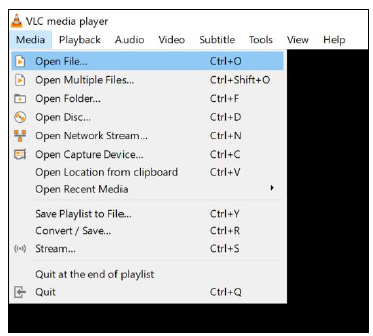
\includegraphics[width=0.5\linewidth]{page10-image-3.png}
\end{figure}
\clearpage
(Q)
Describe: Artificial Intelligence
\clearpage
AI in Music\\ 
\begin{figure}[H]
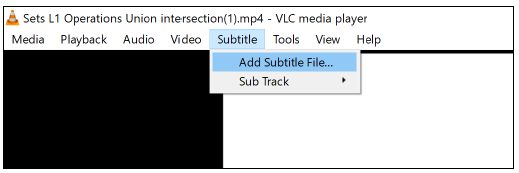
\includegraphics[width=0.5\linewidth]{page10-image-4.png}
\end{figure}
\clearpage
(Q)
Describe: Artificial Intelligence
\clearpage
AI in Agriculture\\ 
\begin{figure}[H]

\includegraphics[width=0.5\linewidth]{page11-image-1.png}
\end{figure}
\clearpage
(Q)
Describe: Artificial Intelligence
\clearpage
AI in Delivery Services\\ 
\begin{figure}[H]

\includegraphics[width=0.5\linewidth]{page11-image-2.png}
\end{figure}
\clearpage
(Q)
Describe: Artificial Intelligence
\clearpage
AI in Self-Driving Vehicles\\ 
\begin{figure}[H]

\includegraphics[width=0.5\linewidth]{page12-image-1.png}
\end{figure}
\clearpage
(Q)
Describe: Artificial Intelligence
\clearpage
AI in Medicine\\ 
\begin{figure}[H]

\includegraphics[width=0.5\linewidth]{page12-image-2.png}
\end{figure}
\clearpage
(Q)
Describe: Artificial Intelligence
\clearpage
AI in Medicine\\ 
\begin{figure}[H]

\includegraphics[width=0.5\linewidth]{page13-image-1.png}
\end{figure}
\clearpage
(Q)
Describe: Artificial Intelligence
\clearpage
AI in Medicine\\ 
\begin{figure}[H]

\includegraphics[width=0.5\linewidth]{page13-image-2.png}
\end{figure}
\clearpage
(Q)
Describe: Artificial Intelligence
\clearpage
AI in Medicine\\ 
\begin{figure}[H]

\includegraphics[width=0.5\linewidth]{page14-image-1.png}
\end{figure}
\clearpage
(Q)
Describe: Artificial Intelligence
\clearpage
AI in Security\\ 
\begin{figure}[H]

\includegraphics[width=0.5\linewidth]{page14-image-2.png}
\end{figure}
\clearpage
(Q)
Describe: Artificial Intelligence
\clearpage
AI in Forensic Identification\\ 
\begin{figure}[H]

\includegraphics[width=0.5\linewidth]{page15-image-1.png}
\end{figure}
\clearpage
(Q)
Describe: AI in Natural Language Processing
\clearpage
• Web search engines\\ 
\section{AI in Natural Language Processing}
46\\
\begin{figure}[H]

\includegraphics[width=0.5\linewidth]{page15-image-2.png}
\end{figure}
\clearpage
(Q)
Describe: AI in Natural Language Processing
\clearpage
Speech Technologies\\ 
\begin{figure}[H]

\includegraphics[width=0.5\linewidth]{page16-image-1.png}
\end{figure}
\clearpage
(Q)
Describe: • 1950: Turing's “Computing 
\clearpage
Brief History of AI\\ 
\section{• 1950: Turing's “Computing }
Machinery and \\
Intelligence”\\
1950-1970: Excitement\\
\end{itemize}
  \item 1950s: Early AI programs: 
Samuel's checkers \\
program, Newell \& \\
Simon's Logic Theorist, \\
Gelernter's Geometry \\
Engine\\
  \item 1956: Dartmouth meeting: 
“Artificial Intelligence” \\
adopted\\
  \item 1965: Robinson's complete 
algorithm for logical \\
reasoning\\
1970-1990: Knowledge-\\
based approaches\\
  \item 1969-79: Early 
development of \\
knowledge-based systems\\
  \item 1980-88: Expert systems
industry booms\\
  \item 1988-93: Expert systems 
industry busts: “AI Winter”\\
Lesson Notes from Nikita Kitaev, University of California, Berkeley\\
\end{itemize}
\begin{figure}[H]

\includegraphics[width=0.5\linewidth]{page16-image-2.png}
\end{figure}
\clearpage
(Q)
Describe: focus on uncertainty
\clearpage
Brief History of AI\\ 
\section{focus on uncertainty}
\begin{itemize}
  \item General increase in technical 
depth\\
  \item Agents and machine learning 
systems… “AI Spring”?\\
2012 – now: \\
Excitement:\\
  \item Big data, big compute, deep 
neural networks\\
  \item Some re-unification of 
subfields\\
  \item AI used in many industries
Lesson Notes from Nikita Kitaev, University of California, Berkeley\\
\end{itemize}
\begin{figure}[H]

\includegraphics[width=0.5\linewidth]{page17-image-1.png}
\end{figure}
\clearpage
(Q)
Describe: Psychology
\clearpage
Foundations of Artificial Intelligence\\ 
\section{Psychology}
Computer \\
engineering\\
Control \\
theory and \\
cybernetics\\
\begin{figure}[H]

\includegraphics[width=0.5\linewidth]{page17-image-2.png}
\end{figure}
\clearpage
(Q)
Describe: Psychology
\clearpage
Questions?\\ 
\begin{figure}[H]
\includegraphics[width=0.5\linewidth]{page17-image-3.png}
\end{figure}
\clearpage
(Q)
Describe: • Oliver Selfridge,
\clearpage
The Thinking Machine\\ 
\section{• Oliver Selfridge,}
\end{itemize}
  \item Claude Shannon
  \item Can a robot marry my daughter?
  \item Can AI translate write poetry?
\end{itemize}
\begin{figure}[H]
\includegraphics[width=0.5\linewidth]{page18-image-1.png}
\end{figure}
\clearpage
(Q)
Describe: • Oliver Selfridge,
\clearpage
Human Intelligence\\ 
\begin{figure}[H]
\includegraphics[width=0.5\linewidth]{page18-image-2.png}
\end{figure}
\clearpage
(Q)
Describe: associate with human  thinking, activities 
\clearpage
Approach 1: Thinking Humanly\\ 
\section{associate with human  thinking, activities }
such as  decision-making, problem \\
solving,  learning ...” (Bellman, 1978)\\
What is Artificial Intelligence?\\
54\\
Artificial Intelligence: A Modern Approach, 2016, Russell \& Norvig\\
\begin{figure}[H]
\includegraphics[width=0.5\linewidth]{page18-image-3.png}
\end{figure}
\clearpage
(Q)
Describe: things at which, at  the moment, people 
\clearpage
Approach 2: Acting Humanly\\ 
\section{things at which, at  the moment, people }
are better.”  (Rich and Knight, 1991)\\
What is Artificial Intelligence?\\
55\\
Artificial Intelligence: A Modern Approach, 2016, Russell \& Norvig\\
\begin{figure}[H]
\includegraphics[width=0.5\linewidth]{page18-image-4.png}
\end{figure}
\clearpage
(Q)
Describe: act.” (Winston, 1992)
\clearpage
Approach 3: Thinking Rationally\\ 
\section{act.” (Winston, 1992)}
What is Artificial Intelligence?\\
56\\
Artificial Intelligence: A Modern Approach, 2016, Russell \& Norvig\\
\begin{figure}[H]
\includegraphics[width=0.5\linewidth]{page18-image-5.png}
\end{figure}
\clearpage
(Q)
Describe: What is Artificial Intelligence?
\clearpage
Approach 4: Acting Rationally\\ 
\section{What is Artificial Intelligence?}
57\\
Artificial Intelligence: A Modern Approach, 2016, Russell \& Norvig\\
\begin{figure}[H]
\includegraphics[width=0.5\linewidth]{page18-image-6.png}
\end{figure}
\clearpage
(Q)
Describe: What is Artificial Intelligence?
\clearpage
Approaches to defining AI\\ 
\begin{figure}[H]
\includegraphics[width=0.5\linewidth]{page18-image-7.png}
\end{figure}
\clearpage
(Q)
Describe: • Cognitive modelling approach
\clearpage
Approaches to defining AI\\ 
\section{• Cognitive modelling approach}
\begin{itemize}
  \item Introspection, psychological  
experiments, brain imaging\\
  \item Cognitive Science
Systems that think rationally\\
Acting Systems that act like humans Systems that act rationally\\
\end{itemize}
\begin{figure}[H]
\includegraphics[width=0.5\linewidth]{page18-image-8.png}
\end{figure}
\clearpage
(Q)
Describe: • Cognitive modelling approach
\clearpage
Approaches to defining AI\\ 
\section{• Cognitive modelling approach}
\end{itemize}
  \item Introspection, psychological  
experiments, brain imaging\\
  \item Cognitive Science
Systems that think rationally\\
  \item Laws of thought approach
  \item “Logicist” tradition
  \item Mostly rule-based
  \item Logic
Acting Systems that act like humans Systems that act rationally\\
\end{itemize}
\begin{figure}[H]
\includegraphics[width=0.5\linewidth]{page18-image-9.png}
\end{figure}
\clearpage
(Q)
Describe: • Cognitive modelling approach
\clearpage
Approaches to defining AI\\ 
\section{• Cognitive modelling approach}
\begin{itemize}
  \item Introspection, psychological  
experiments, brain imaging\\
  \item Cognitive Science
Systems that think rationally\\
  \item Laws of thought approach
  \item “Logicist” tradition
  \item Mostly rule-based
  \item Logic
Acting\\
Systems that act like humans\\
  \item The (total) Turing Test
  \item Requires the 6 disciplines
  \item NLP, KR, Reasoning, ML,  
Computer vision, Robotics\\
Systems that act rationally\\
\end{itemize}
\begin{figure}[H]
\includegraphics[width=0.5\linewidth]{page18-image-10.png}
\end{figure}
\clearpage
(Q)
Describe: • Cognitive modelling approach
\clearpage
Approaches to defining AI\\ 
\section{• Cognitive modelling approach}
\end{itemize}
  \item Introspection, psychological  
experiments, brain imaging\\
  \item Cognitive Science
Systems that think rationally\\
  \item Laws of thought approach
  \item “Logicist” tradition
  \item Mostly rule-based
  \item Logic
Acting\\
Systems that act like humans\\
  \item The (total) Turing Test
  \item Requires the 6 disciplines
  \item NLP, KR, Reasoning, ML,  
Computer vision, Robotics\\
Systems that act rationally\\
  \item The rational agent approach
  \item Autonomous, perceptive,  
persistent, adapts to change\\
  \item Creates and pursues goals
\end{itemize}
\begin{figure}[H]
\includegraphics[width=0.5\linewidth]{page19-image-1.png}
\end{figure}
\clearpage
(Q)
Describe: • Cognitive modelling approach
\clearpage
Approaches to defining AI\\ 
\section{• Cognitive modelling approach}
\begin{itemize}
  \item Introspection, psychological  
experiments, brain imaging\\
  \item Cognitive Science
Systems that think rationally\\
  \item Laws of thought approach
  \item “Logicist” tradition
  \item Mostly rule-based
  \item Logic
Acting\\
Systems that act like humans\\
  \item The (total) Turing Test
  \item Requires the 6 disciplines
  \item NLP, KR, Reasoning, ML,  
Computer vision, Robotics\\
Systems that act rationally\\
  \item The rational agent approach
  \item Autonomous, perceptive,  
persistent, adapts to change\\
  \item Creates and pursues goals
\end{itemize}
\begin{figure}[H]
\includegraphics[width=0.5\linewidth]{page19-image-2.png}
\end{figure}
\clearpage
(Q)
Describe: • makes appropriate choices given perceptual and computational limitations
\clearpage
An agent ‘acts’ (does something) within an environment\\ 
\section{• makes appropriate choices given perceptual and computational limitations}
What is an Agent?\\
64\\
Artificial Intelligence: Foundations of Computational Agents, 2017, Poole \& Markworth\\
\begin{figure}[H]
\includegraphics[width=0.5\linewidth]{page19-image-3.png}
\end{figure}
\clearpage
(Q)
Describe: • Computers (“hardware”)
\clearpage
A computational agent is:\\ 
\section{• Computers (“hardware”)}
\end{itemize}
  \item Non computational agents:
  \item wind, rain, etc.
Computational Agent\\
\end{itemize}
65\\
Artificial Intelligence: Foundations of Computational Agents, 2017, Poole \& Markworth\\
\begin{figure}[H]
\includegraphics[width=0.5\linewidth]{page20-image-1.png}
\end{figure}
\clearpage
(Q)
Describe: behaviour
\clearpage
• Rational agent acts to ‘achieve the best outcome or, when there is  uncertainty, the \\ 
\section{behaviour}
\begin{itemize}
  \item It is more general than the “laws of thought” approach
  \item Also deals with limited rationality – acting appropriately with limited computations
Rational Agent\\
\end{itemize}
66\\
Artificial Intelligence: A Modern Approach, 2016, Russell \& Norvig\\
\begin{figure}[H]
\includegraphics[width=0.5\linewidth]{page20-image-2.png}
\end{figure}
\clearpage
(Q)
Describe: • makes appropriate choices given perceptual and computational  limitations
\clearpage
• AI is the field that studies the synthesis and analysis of computational agents that \\ 
\section{• makes appropriate choices given perceptual and computational  limitations}
Intelligence\\
67\\
Artificial Intelligence: Foundations of Computational Agents, 2017, Poole \& Markworth\\
\begin{figure}[H]
\includegraphics[width=0.5\linewidth]{page20-image-3.png}
\end{figure}
\clearpage
(Q)
Describe: • makes appropriate choices given perceptual and computational  limitations
\clearpage
• AI is the field that studies the synthesis and analysis of computational agents that \\ 
\section{• makes appropriate choices given perceptual and computational  limitations}
Intelligence\\
68\\
Artificial Intelligence: Foundations of Computational Agents, 2017, Poole \& Markworth\\
\begin{figure}[H]
\includegraphics[width=0.5\linewidth]{page20-image-4.png}
\end{figure}
\clearpage
(Q)
Describe: Artificial Intelligence: Foundations of Computational Agents, 2017, Poole \& Markworth
\clearpage
Artificial intelligence, or AI is the field that studies the \\ 
\section{Artificial Intelligence: Foundations of Computational Agents, 2017, Poole \& Markworth}
\begin{figure}[H]
\includegraphics[width=0.5\linewidth]{page21-image-1.png}
\end{figure}
\clearpage
(Q)
Describe: Artificial Intelligence: Foundations of Computational Agents, 2017, Poole \& Markworth
\clearpage
Questions?\\ 
\begin{figure}[H]
\includegraphics[width=0.5\linewidth]{page21-image-2.png}
\end{figure}
\clearpage
(Q)
Describe: • Focuses on building empirical systems
\clearpage
Two types of goals: Scientific and Engineering\\ 
\section{• Focuses on building empirical systems}
\end{itemize}
  \item And not on the final applications that could be deployed to use
Goals of AI\\
\end{itemize}
71\\
Artificial Intelligence: Foundations of Computational Agents, 2017, Poole \& Markworth\\
\begin{figure}[H]
\includegraphics[width=0.5\linewidth]{page21-image-3.png}
\end{figure}
\clearpage
(Q)
Describe: 72
\clearpage
Two types of goals: Scientific and Engineering\\ 
\section{72}
Artificial Intelligence: Foundations of Computational Agents, 2017, Poole \& Markworth\\
\begin{figure}[H]
\includegraphics[width=0.5\linewidth]{page21-image-4.png}
\end{figure}
\clearpage
(Q)
Describe: • Better predictions \& improved decision making
\clearpage
• Workflow/Process automation\\ 
\section{• Better predictions \& improved decision making}
\begin{itemize}
  \item Predictions of risks, performance targets, tailored product offerings etc
Business Benefits of AI\\
\end{itemize}
73\\
\begin{figure}[H]
\includegraphics[width=0.5\linewidth]{page22-image-1.png}
\end{figure}
\clearpage
(Q)
Describe: • Agriculture
\clearpage
• Healthcare\\ 
\section{• Agriculture}
\end{itemize}
  \item Real-time data analytics help farmers to maximise their crop yields and  profits
  \item Overall lifestyle
Social benefits of AI\\
\end{itemize}
74\\
\begin{figure}[H]
\includegraphics[width=0.5\linewidth]{page22-image-2.png}
\end{figure}
\clearpage
(Q)
Describe: • Explainable (or Interpretable) AI (XAI)
\clearpage
• Safety and security\\ 
\section{• Explainable (or Interpretable) AI (XAI)}
\begin{itemize}
  \item Deep neural models are naturally opaque
  \item Possible job losses
  \item “AI will replace more than 75 million jobs by 2022” – World Economic Forum
Risks and Challenges of AI\\
\end{itemize}
75\\
\begin{figure}[H]
\includegraphics[width=0.5\linewidth]{page23-image-1.png}
\end{figure}
\clearpage
(Q)
Describe: • IBM abandons “biased” facial recognition tech – BBC
\clearpage
• Accountability\\ 
\section{• IBM abandons “biased” facial recognition tech – BBC}
\end{itemize}
  \item Technological social responsibility (TSR)
  \item a conscious alignment between short- and medium-term business goals and  
longer-term societal ones – McKinsey Quarterly, August, 2019\\
Ethical Concerns of AI\\
\end{itemize}
76\\
\begin{figure}[H]
\includegraphics[width=0.5\linewidth]{page23-image-2.png}
\end{figure}
\clearpage
(Q)
Describe: • Risk and Challenges
\clearpage
• Artificial Intelligence: An overview\\ 
\section{• Risk and Challenges}
\begin{itemize}
  \item Ethical Issues
AI Summary\\
\end{itemize}
77\\
\begin{figure}[H]
\includegraphics[width=0.5\linewidth]{page24-image-1.png}
\end{figure}
\clearpage
(Q)
Describe: • Risk and Challenges
\clearpage
Questions?\\ 
\begin{figure}[H]
\includegraphics[width=0.5\linewidth]{page24-image-2.png}
\end{figure}
\clearpage
(Q)
Describe: • Risk and Challenges
\clearpage
SCC361: Artificial Intelligence\\ 
\begin{figure}[H]
\includegraphics[width=0.5\linewidth]{page25-image-1.png}
\end{figure}
\clearpage
(Q)
Describe: • Supervised Learning
\clearpage
• Overview of Machine Learning\\ 
\section{• Supervised Learning}
\end{itemize}
  \item Classification and regression
  \item Unsupervised Learning
  \item Clustering and association
Introduction to Machine Learning\\
\end{itemize}
80\\
\begin{figure}[H]
\includegraphics[width=0.5\linewidth]{page25-image-2.png}
\end{figure}
\clearpage
(Q)
Describe: • a subset of ML with additional layers to  
\clearpage
• AI systems were mostly rule-based\\ 
\section{• a subset of ML with additional layers to  }
learn deeper representations data\\
AI and Machine Learning\\
81\\
Artificial Intelligence\\
Machine Learning\\
Deep Learning\\
\begin{figure}[H]
\includegraphics[width=0.5\linewidth]{page26-image-1.png}
\end{figure}
\clearpage
(Q)
Describe: • Inverted alpha-beta pruning widely used in decision 
\clearpage
Early definition of machine learning\\ 
\section{• Inverted alpha-beta pruning widely used in decision }
tree searching\\
What is Machine Learning?\\
82\\
\begin{figure}[H]
\includegraphics[width=0.5\linewidth]{page26-image-2.png}
\end{figure}
\clearpage
(Q)
Describe: • Again, the key is learning from experience
\clearpage
Another popular definition:\\ 
\section{• Again, the key is learning from experience}
\begin{itemize}
  \item Not explicitly programmed
What is Machine Learning?\\
\end{itemize}
83\\
\begin{figure}[H]
\includegraphics[width=0.5\linewidth]{page26-image-3.png}
\end{figure}
\clearpage
(Q)
Describe: • Again, the key is learning from experience
\clearpage
What is Machine Learning?\\ 
\begin{figure}[H]
\includegraphics[width=0.5\linewidth]{page27-image-1.png}
\end{figure}
\clearpage
(Q)
Describe: a. Watching me label emails as spam
\clearpage
Given this definition:\\ 
\section{a. Watching me label emails as spam}
b. Classifying emails as spam or not spam\\
c. The fraction of emails correctly classified as spam or not\\
d. None of the above – this is not a machine learning problem\\
Spam or not SPAM\\
85\\
\begin{figure}[H]
\includegraphics[width=0.5\linewidth]{page27-image-2.png}
\end{figure}
\clearpage
(Q)
Describe: Data ( 𝑥𝑥 )
\clearpage
• Consider the function 𝑦𝑦 = 𝑓𝑓(𝑥𝑥) (e.g. 𝑓𝑓 𝑥𝑥 = 𝑥𝑥 )\\ 
\section{Data ( 𝑥𝑥 )}
Program ( 𝑦𝑦 = 𝑥𝑥 )\\
Output ( 𝑥𝑥 )\\
Computer\\
Data ( 𝑥𝑥 )\\
Output ( 𝑥𝑥 )\\
Program ( 𝑦𝑦 = 𝑥𝑥 )\\
\begin{figure}[H]
\includegraphics[width=0.5\linewidth]{page27-image-3.png}
\end{figure}
\clearpage
(Q)
Describe: Data ( 𝑥𝑥 )
\clearpage
• Consider the function 𝑦𝑦 = 𝑓𝑓(𝑥𝑥) (e.g. 𝑓𝑓 𝑥𝑥 = 𝑥𝑥 )\\ 
\section{Data ( 𝑥𝑥 )}
Program ( 𝑦𝑦 = 𝑥𝑥 )\\
Output ( 𝑥𝑥 )\\
Computer\\
Data ( 𝑥𝑥 )\\
Output ( 𝑥𝑥 )\\
Program ( 𝑦𝑦 = 𝑥𝑥 )\\
\begin{figure}[H]
\includegraphics[width=0.5\linewidth]{page27-image-4.png}
\end{figure}
\clearpage
(Q)
Describe: 88
\clearpage
• Memorization\\ 
\section{88}
Declarative knowledge\\
\begin{figure}[H]
\includegraphics[width=0.5\linewidth]{page27-image-5.png}
\end{figure}
\clearpage
(Q)
Describe: • Deduce new facts from old facts
\clearpage
• Memorization\\ 
\section{• Deduce new facts from old facts}
\end{itemize}
  \item Limited by accuracy of deduction process
  \item Essentially a predictive activity
  \item Assumes that the past predicts the future
How things are learned\\
\end{itemize}
89\\
Imperative knowledge\\
Declarative knowledge\\
\begin{figure}[H]
\includegraphics[width=0.5\linewidth]{page27-image-6.png}
\end{figure}
\clearpage
(Q)
Describe: Types of Machine Learning
\clearpage
Supervised Learning\\ 
\section{Types of Machine Learning}
90\\
\begin{figure}[H]
\includegraphics[width=0.5\linewidth]{page27-image-7.png}
\end{figure}
\clearpage
(Q)
Describe: new unseen data
\clearpage
• The algorithm learns to map an input to a \\ 
\section{new unseen data}
\begin{itemize}
  \item Two broad categories:
  \item Regression
  \item Classification
Supervised Learning\\
\end{itemize}
91\\
\begin{figure}[H]
\includegraphics[width=0.5\linewidth]{page27-image-8.png}
\end{figure}
\clearpage
(Q)
Describe: new unseen data
\clearpage
Supervised Learning\\ 
\begin{figure}[H]
\includegraphics[width=0.5\linewidth]{page27-image-9.png}
\end{figure}
\clearpage
(Q)
Describe: categories (or classes or labels)
\clearpage
• Learns from labelled data (supervised)\\ 
\section{categories (or classes or labels)}
Classification\\
93\\
\begin{figure}[H]
\includegraphics[width=0.5\linewidth]{page27-image-10.png}
\end{figure}
\clearpage
(Q)
Describe: • Typically fits some linear or quadratic curve  of 
\clearpage
• Learns from labelled data (supervised)\\ 
\section{• Typically fits some linear or quadratic curve  of }
the data plot\\
\end{itemize}
  \item Linear or logistic regression algorithms are often 
used\\
Regression\\
\end{itemize}
94\\
\begin{figure}[H]
\includegraphics[width=0.5\linewidth]{page28-image-1.png}
\end{figure}
\clearpage
(Q)
Describe: accuracy is achieved
\clearpage
• Input data = training data\\ 
\section{accuracy is achieved}
\begin{itemize}
  \item Problem types: Classification and Regression
  \item Algorithms:
  \item Logistic Regression
  \item Back Propagation Neural Network.
Supervised Learning Algorithms\\
\end{itemize}
95\\
\begin{figure}[H]
\includegraphics[width=0.5\linewidth]{page28-image-2.png}
\end{figure}
\clearpage
(Q)
Describe: b. Both are classification problems
\clearpage
• If we wish to learn models to address the following\\ 
\section{b. Both are classification problems}
c. Problem 1 is regression while Problem 2 is classification\\
d. Problem 2 is regression while Problem 1 is classification\\
Quiz: Classification vs Regression\\
96\\
\begin{figure}[H]
\includegraphics[width=0.5\linewidth]{page28-image-3.png}
\end{figure}
\clearpage
(Q)
Describe: of the data
\clearpage
• Remember the function 𝑦𝑦 = 𝑓𝑓 𝑥𝑥\\ 
\section{of the data}
\end{itemize}
  \item Two main categories
  \item Clustering
  \item Association
Unsupervised Learning\\
\end{itemize}
97\\
\begin{figure}[H]
\includegraphics[width=0.5\linewidth]{page29-image-1.png}
\end{figure}
\clearpage
(Q)
Describe: of the data
\clearpage
Unsupervised Learning\\ 
\begin{figure}[H]
\includegraphics[width=0.5\linewidth]{page29-image-2.png}
\end{figure}
\clearpage
(Q)
Describe: portions of your data
\clearpage
• In a clustering problem, we want to  discover \\ 
\section{portions of your data}
\begin{itemize}
  \item E.g. people that buy 𝑿𝑿 also tend to buy 𝒀𝒀
Clustering and Association\\
\end{itemize}
99\\
\begin{figure}[H]
\includegraphics[width=0.5\linewidth]{page29-image-3.png}
\end{figure}
\clearpage
(Q)
Describe: • Problem types: clustering, dimensionality  reduction 
\clearpage
• Input data in not labelled\\ 
\section{• Problem types: clustering, dimensionality  reduction }
and association rule learning\\
\end{itemize}
  \item Algorithms:
  \item K-Means algorithm
  \item Apriori algorithm.
Unsupervised Learning Algorithms\\
\end{itemize}
10\\
0\\
\begin{figure}[H]
\includegraphics[width=0.5\linewidth]{page30-image-1.png}
\end{figure}
\clearpage
(Q)
Describe: • Many real world problems adopt this method
\clearpage
• Semi-supervised learning approach refers to:\\ 
\section{• Many real world problems adopt this method}
\begin{itemize}
  \item It can be expensive or time-consuming to label data
  \item A hybrid design often helps to bridge the gaps
  \item Algorithms:
  \item A flexible combination of supervised and unsupervised 
algorithms\\
Semi-supervised Learning\\
\end{itemize}
10\\
1\\
\begin{figure}[H]
\includegraphics[width=0.5\linewidth]{page30-image-2.png}
\end{figure}
\clearpage
(Q)
Describe: supervised
\clearpage
Today’s Lecture\\ 
\section{supervised}
\end{itemize}
  \item Supervised Learning
  \item Classification and regression
  \item Unsupervised Learning
  \item Clustering and association
Machine Learning Summary\\
\end{itemize}
10\\
2\\
\begin{figure}[H]
\includegraphics[width=0.5\linewidth]{page30-image-3.png}
\end{figure}
\clearpage
(Q)
Describe: SCC361/P01/01 Wednesday 11:00-13:00 FST B076
\clearpage
Labs: Introduction to Matlab\\ 
\section{SCC361/P01/01 Wednesday 11:00-13:00 FST B076}
SCC361/P01/02 Thursday 16:00-18:00 FST B076\\
SCC361/P01/03 Friday 16:00-18:00 FST B070\\
SCC361/P01/04 Thursday 10:00-12:00 FST B070\\
SCC361/P01/05 Friday 11:00-13:00 FST B080\\
\begin{figure}[H]
\includegraphics[width=0.5\linewidth]{page31-image-1.png}
\end{figure}
\clearpage
(Q)
Describe: 10
\clearpage
Labs: Introduction to Matlab\\ 
\section{10}
4\\
Group Day Time Room\\
SCC361/P01/01 Wednesday 11:00-13:00 FST B076\\
SCC361/P01/02 Thursday 16:00-18:00 FST B076\\
SCC361/P01/03 Friday 16:00-18:00 FST B070\\
SCC361/P01/04 Thursday 10:00-12:00 FST B070\\
SCC361/P01/05 Friday 11:00-13:00 FST B080\\
\begin{figure}[H]
\includegraphics[width=0.5\linewidth]{page31-image-2.png}
\end{figure}
\clearpage
(Q)
Describe: 10
\clearpage
Questions?\\ 
\begin{figure}[H]
\includegraphics[width=0.5\linewidth]{page31-image-3.png}
\end{figure}
\clearpage
(Q)
Describe: 10
\clearpage
\clearpage
(Q)
Describe: 10
\clearpage
\\ 
\end{document}